\documentclass{ctexart}
\CTEXsetup[format={\Large\bfseries}]{section}            % 让section靠左对齐
\usepackage{graphicx} % Required for inserting images
\usepackage{enumerate} % 下面1,2,3小点


% 设置 subsection 的间距
\usepackage{titlesec}
\titlespacing{\section}{0pt}{0.75\baselineskip}{0.75\baselineskip}
\titlespacing{\subsection}{0pt}{0.5\baselineskip}{0.5\baselineskip}

\usepackage{geometry} % 调整页边距和纸张大小
\geometry{a4paper,scale=0.7} 

\title{\vspace{-2cm}\textbf{程序设计基础课程设计报告} \\ \fontsize{12}{14}{---动态链表}}

\author{高宇轩 23009200132}
\date{\today}

\begin{document}
    
    \maketitle
    
    \section{原始题目及要求}
    链表是一种重要的数据结构,需要动态的进行存储分配,要求通过函数分别实现动态链表的建立、结点的插入、结点的删除以及链表的输出。
    
    \section{题目分析}
    
    \subsection{题目功能}
    通过动态的存储分配实现链表。
    
    链表能够被建立,能够在尾部插入元素,能够删除某一个元素,能够打印链表的内容,能够查找某个元素是否在链表中。
    \subsection{题目知识点}
    内存管理、结构体定义、指针运用、函数
    
    \section{题目总体方案设计}
    
    \begin{figure}[h] % 'h' 表示将图片放置在当前位置
       \centering
       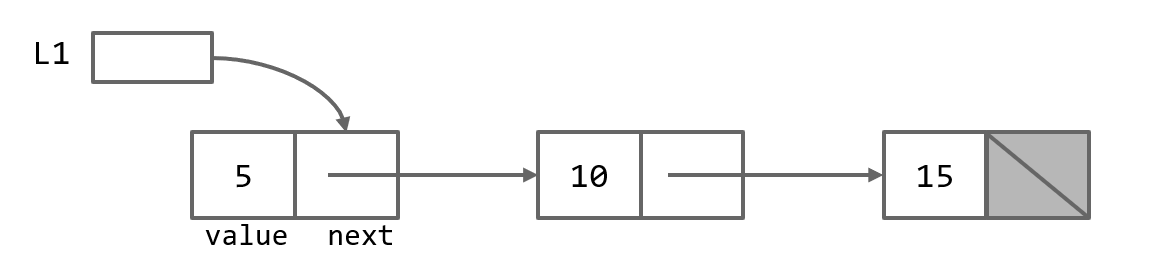
\includegraphics[width=0.8\textwidth]{LinkedList.png}
       \caption{链表示意图}   
    \end{figure}
    
    
    \begin{figure}[h] % 'h' 表示将图片放置在当前位置
        \centering
        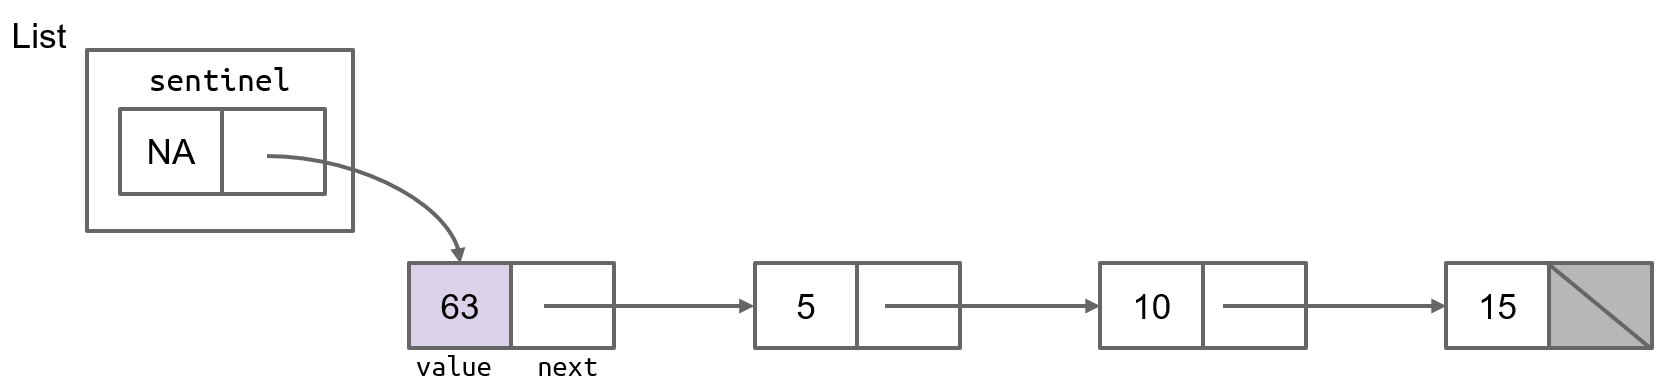
\includegraphics[width=0.8\textwidth]{sentinel.png}
        \caption{增加哨兵节点后的链表示意图}   
    \end{figure}

    
    
    \section{各功能模块的设计说明}
    \subsection{链表建立}
    基于我们的哨兵节点,建立链表的操作相当于初始化一个哨兵节点。
    
    \subsection{插入元素}
    插入元素,要先把插入节点的next成员设置为前一个结点原来的next成员,然后将前一个节点的next成员设置为新插入的节点。
    
    \subsection{删除元素}
    先找到要删除元素对应的节点,然后用一个游标跟踪前一个结点,将前一个节点的next成员直接设置为删除节点的next,此时需要删除的节点就不在链表中了,同时要释放删除节点的内存,防止内存泄漏。
    
    
    \subsection{打印链表}
    遍历一遍链表,同时将每一个节点的value成员输出。
    
    \subsection{清除内存}
    遍历所有的节点,然后将每一个节点分配的内存释放,防止出现内存泄漏。
    
    \section{程序的集成测试}
    图3中的操作调用了链表的所有功能,通过图4中链表输出的结果,我们可以看出链表的操作满足了我们的要求。
    \begin{figure}[h] % 'h' 表示将图片放置在当前位置
       \centering
       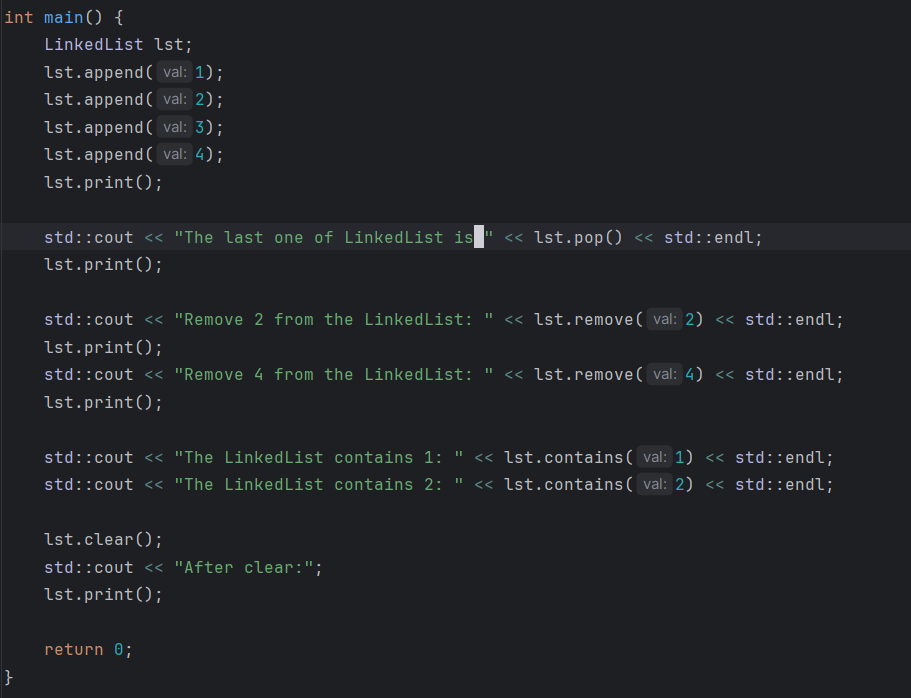
\includegraphics[width=0.7\textwidth]{test1.png}
       \caption{程序的集成测试内容}
    \end{figure}
    
    \begin{figure}[h] % 'h' 表示将图片放置在当前位置
        \centering
        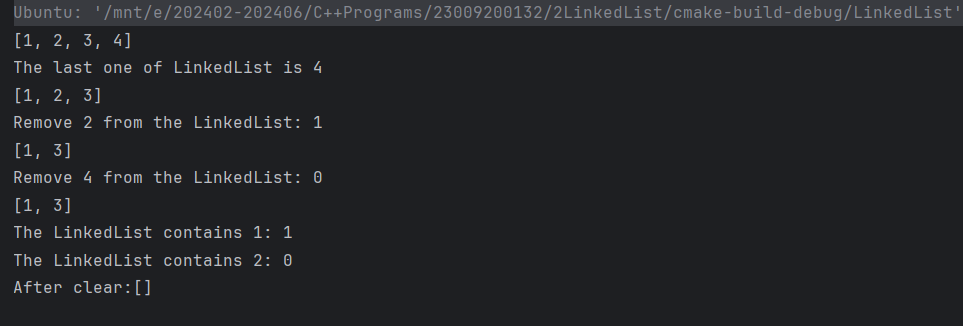
\includegraphics[width=0.7\textwidth]{test2.png}
        \caption{程序的集成测试结果}
    \end{figure}
    
    \section{总结}
    根据程序的集成测试,可以看出我们的链表操作符合程序的需求。
    
    另外,为了提高链表的效率,我们还可以设置尾指针作为标识,提高查询,插入或删除尾部元素的操作。此时我们可以类比头部的哨兵节点,设置尾部的哨兵节点来减少空链表情况下的讨论,或者采用循环链表的方式进行简化。
    
    
\end{document}
